\PassOptionsToPackage{unicode=true}{hyperref} % options for packages loaded elsewhere
\PassOptionsToPackage{hyphens}{url}
%
\documentclass[10pt,ignorenonframetext,]{beamer}
\usepackage{pgfpages}
\setbeamertemplate{caption}[numbered]
\setbeamertemplate{caption label separator}{: }
\setbeamercolor{caption name}{fg=normal text.fg}
\beamertemplatenavigationsymbolsempty
% Prevent slide breaks in the middle of a paragraph:
\widowpenalties 1 10000
\raggedbottom
\setbeamertemplate{part page}{
\centering
\begin{beamercolorbox}[sep=16pt,center]{part title}
  \usebeamerfont{part title}\insertpart\par
\end{beamercolorbox}
}
\setbeamertemplate{section page}{
\centering
\begin{beamercolorbox}[sep=12pt,center]{part title}
  \usebeamerfont{section title}\insertsection\par
\end{beamercolorbox}
}
\setbeamertemplate{subsection page}{
\centering
\begin{beamercolorbox}[sep=8pt,center]{part title}
  \usebeamerfont{subsection title}\insertsubsection\par
\end{beamercolorbox}
}
\AtBeginPart{
  \frame{\partpage}
}
\AtBeginSection{
  \ifbibliography
  \else
    \frame{\sectionpage}
  \fi
}
\AtBeginSubsection{
  \frame{\subsectionpage}
}
\usepackage{lmodern}
\usepackage{amssymb,amsmath}
\usepackage{ifxetex,ifluatex}
\usepackage{fixltx2e} % provides \textsubscript
\ifnum 0\ifxetex 1\fi\ifluatex 1\fi=0 % if pdftex
  \usepackage[T1]{fontenc}
  \usepackage[utf8]{inputenc}
  \usepackage{textcomp} % provides euro and other symbols
\else % if luatex or xelatex
  \usepackage{unicode-math}
  \defaultfontfeatures{Ligatures=TeX,Scale=MatchLowercase}
\fi
\usetheme[]{Luebeck}
\usecolortheme{whale}
\usefonttheme{structuresmallcapsserif}
% use upquote if available, for straight quotes in verbatim environments
\IfFileExists{upquote.sty}{\usepackage{upquote}}{}
% use microtype if available
\IfFileExists{microtype.sty}{%
\usepackage[]{microtype}
\UseMicrotypeSet[protrusion]{basicmath} % disable protrusion for tt fonts
}{}
\IfFileExists{parskip.sty}{%
\usepackage{parskip}
}{% else
\setlength{\parindent}{0pt}
\setlength{\parskip}{6pt plus 2pt minus 1pt}
}
\usepackage{hyperref}
\hypersetup{
            pdfauthor={Luisa Hammer and Marcelo Avila},
            pdfborder={0 0 0},
            breaklinks=true}
\urlstyle{same}  % don't use monospace font for urls
\newif\ifbibliography
\usepackage{longtable,booktabs}
\usepackage{caption}
% These lines are needed to make table captions work with longtable:
\makeatletter
\def\fnum@table{\tablename~\thetable}
\makeatother
\usepackage{graphicx,grffile}
\makeatletter
\def\maxwidth{\ifdim\Gin@nat@width>\linewidth\linewidth\else\Gin@nat@width\fi}
\def\maxheight{\ifdim\Gin@nat@height>\textheight\textheight\else\Gin@nat@height\fi}
\makeatother
% Scale images if necessary, so that they will not overflow the page
% margins by default, and it is still possible to overwrite the defaults
% using explicit options in \includegraphics[width, height, ...]{}
\setkeys{Gin}{width=\maxwidth,height=\maxheight,keepaspectratio}
\setlength{\emergencystretch}{3em}  % prevent overfull lines
\providecommand{\tightlist}{%
  \setlength{\itemsep}{0pt}\setlength{\parskip}{0pt}}
\setcounter{secnumdepth}{0}

% set default figure placement to htbp
\makeatletter
\def\fps@figure{htbp}
\makeatother

\widowpenalties 1 150
\newcommand{\begincols}[1]{\begin{columns}{#1}}
\newcommand{\stopcols}{\end{columns}}

\title{Replication of ``Educational Expansion and Its Heterogeneous Returns for
Wage Workers''\\
by\\
Michael Gebel and Friedhelm Pfeiffer}
\author{Luisa Hammer and Marcelo Avila}
\date{22 Nov 2018}

\begin{document}
\frame{\titlepage}

\hypertarget{introduction}{%
\section{Introduction}\label{introduction}}

\begin{frame}{L: Outline}
\protect\hypertarget{l-outline}{}

\begin{itemize}
\item
  Theoretical Framework

  \begin{itemize}
  \tightlist
  \item
    Gebel \& Pfeiffer (2010)
  \item
    Returns to education
  \end{itemize}
\item
  Empirical framework

  \begin{itemize}
  \tightlist
  \item
    Correlated random coefficients model
  \item
    Conditional Mean approach
  \item
    Control funtion approach
  \end{itemize}
\item
  Replication

  \begin{itemize}
  \tightlist
  \item
    Set-up
  \item
    Code
  \item
    Comparison of results
  \end{itemize}
\end{itemize}

\end{frame}

\hypertarget{theoretical-framework}{%
\subsection{Theoretical Framework}\label{theoretical-framework}}

\begin{frame}{L: Summary of Gebel and Pfeiffer (2010)}
\protect\hypertarget{l-summary-of-gebel-and-pfeiffer-2010}{}

\begin{itemize}
\item
  Basic idea: examine evolution of returns to education in West German
  labour market.
\item
  Focus on change in returns to education over time as a consequence to
  education expansion in Germany.
\item
  methodology:

  \begin{itemize}
  \tightlist
  \item
    Wooldrigdge's (2004) \textbf{conditional mean independence}
  \item
    Garen's (1984) \textbf{control function} approach, that requires an
    \emph{exclusion restriction}
  \item
    as well as OLS regression
  \end{itemize}
\item
  data: SOEP 1984-2006
\end{itemize}

\end{frame}

\begin{frame}[allowframebreaks]{L: Background Information}
\protect\hypertarget{l-background-information}{}

\textbf{Increase in educational attainment}

\begin{figure}
\centering
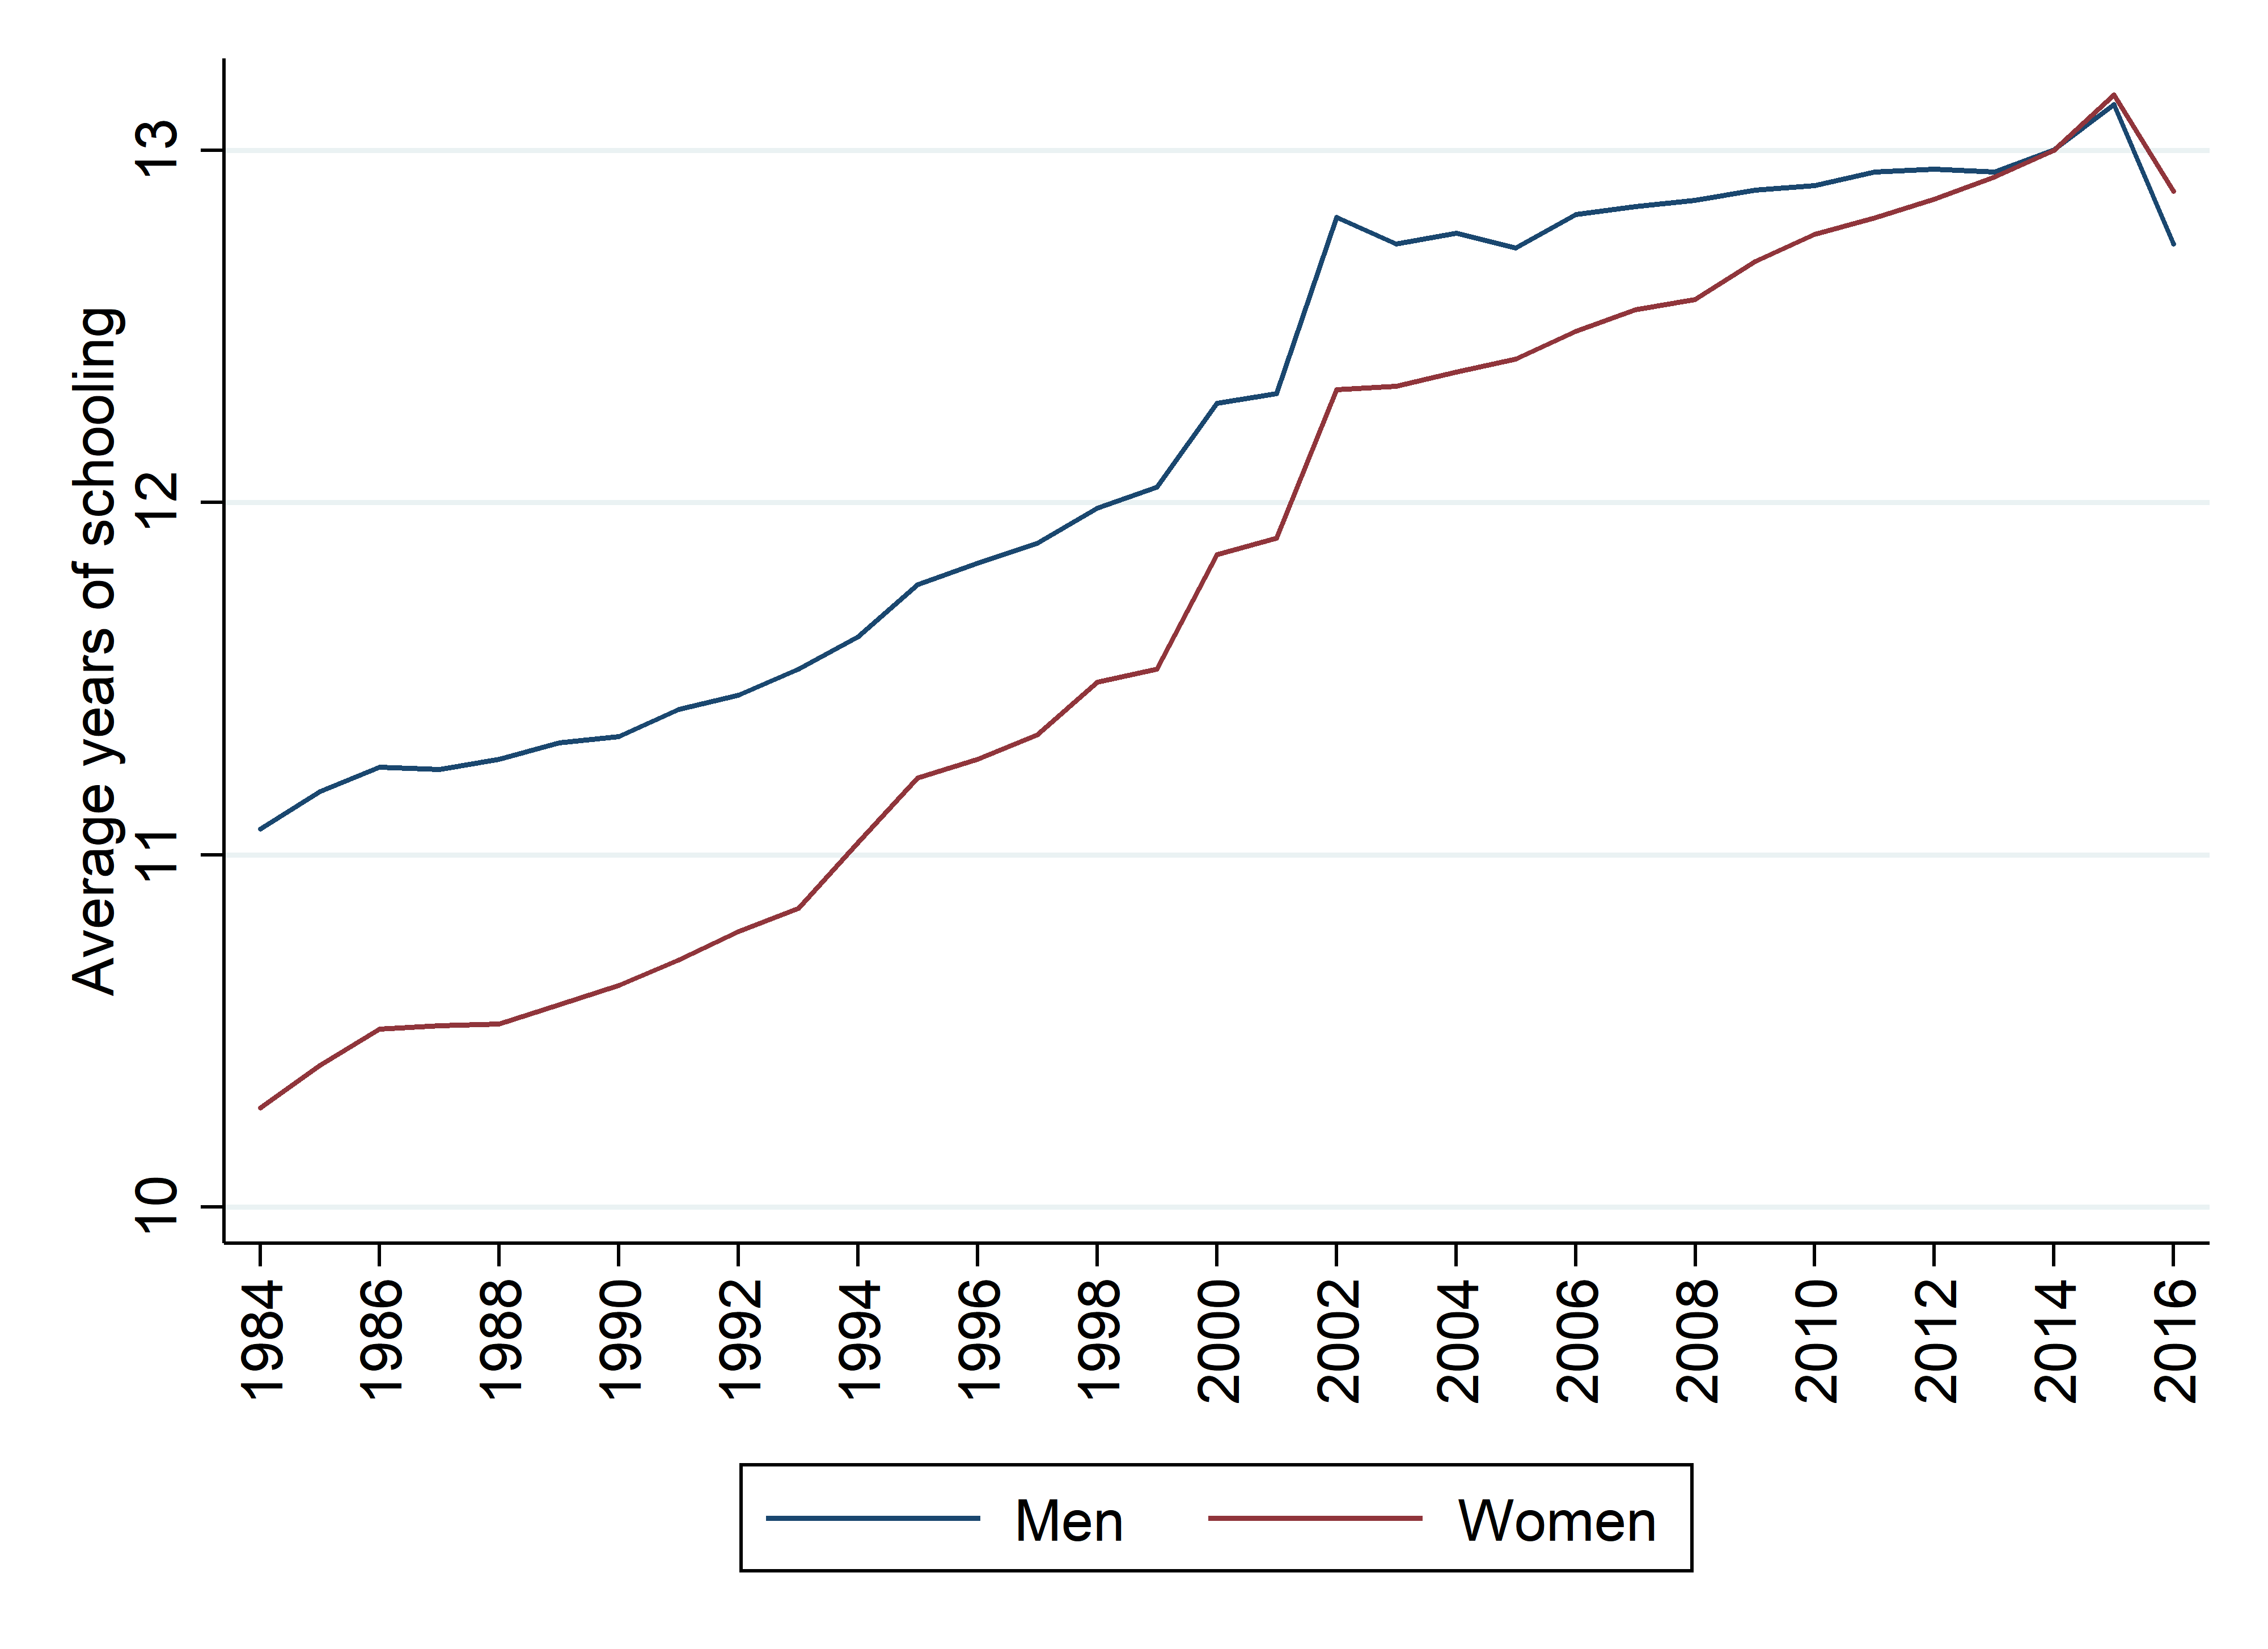
\includegraphics[width=\textwidth,height=2.08333in]{img/edu_sex.png}
\caption{Source: SOEP 1984-2016, own estimations.}
\end{figure}

\textbf{How can educational expansion affect the returns to education?}

\begin{itemize}
\tightlist
\item
  Standard theory: an increase of labor supply of high-skilled workers
  should decrease the returns to education
\item
  High-educated workers with higher unobserved motivation / ability
  which positively affects wages
\item
  If more less talented are accepted to higher education, this should
  decrease the average productivity levels of higher educated workers
  --\textgreater{} overall effect not clear
\end{itemize}

\textbf{Problems in the estimation of returns to education}

\begin{itemize}
\tightlist
\item
  unobserved characteristics leading to \textbf{selection bias}:

  \begin{itemize}
  \tightlist
  \item
    higher ability and motivation to stay longer in education.
  \item
    select jobs with higher expected returns.
  \end{itemize}
\end{itemize}

\end{frame}

\hypertarget{econometric-approach}{%
\subsection{Econometric Approach}\label{econometric-approach}}

\begin{frame}[allowframebreaks]{M: Empirical Framework (Derivation)}
\protect\hypertarget{m-empirical-framework-derivation}{}

The study is based on the \textbf{correlated random coefficient model}
(Wooldridge, 2004) specified as: \[\ln Y_i = a_i + b_i S_i\] with
\(a_i = a'X_i + \varepsilon_{ai}\), and
\(b_i = b'X_i + \varepsilon_{bi}\)

where \(\ln Y_i\) : log of wages and \(S_i\) years of schooling of
individual \(i\)

\begin{itemize}
\item
  The model has, therefore, an \textbf{individual-specific intercept}
  \(a_i\) and \textbf{slope} \(b_i\) dependent on \textbf{observables}
  \(X_i\) and \textbf{unobservables} \(\varepsilon_{ai}\) and
  \(\varepsilon_{bi}\).
\item
  Do not assume that \(b_i\) and \(S_i\) are independent
  --\textgreater{} Individuals with higher expected benefits from
  education are more likely to remain longer in education
  --\textgreater{} \(b_i\) may be correlated with \(S_i\) indicating
  positive self-selection.
\item
  focus: estimate average partial effect (APE), which is the return per
  additional year of education for a randomly chosen individual (or
  averaged across the population)
  \[E(\partial \ln Y / \partial S) = E(b_i) = \beta\]
\end{itemize}

In case of homogeneous returns to education the wage equation reduces
to: \[\ln Y_i = a'X_i + \bar b S_i + \varepsilon_{ai}\]

\begin{itemize}
\item
  Unobserved heterogeneity may only affect the \textbf{intercept} of the
  wage equation.
\item
  still potential endogeneity if \(\varepsilon_{ai}\) correlates with
  \(S_i\)
\end{itemize}

\end{frame}

\begin{frame}{M: Empirical Framework (Intuition) I\}}
\protect\hypertarget{m-empirical-framework-intuition-i}{}

\begin{figure}
\centering
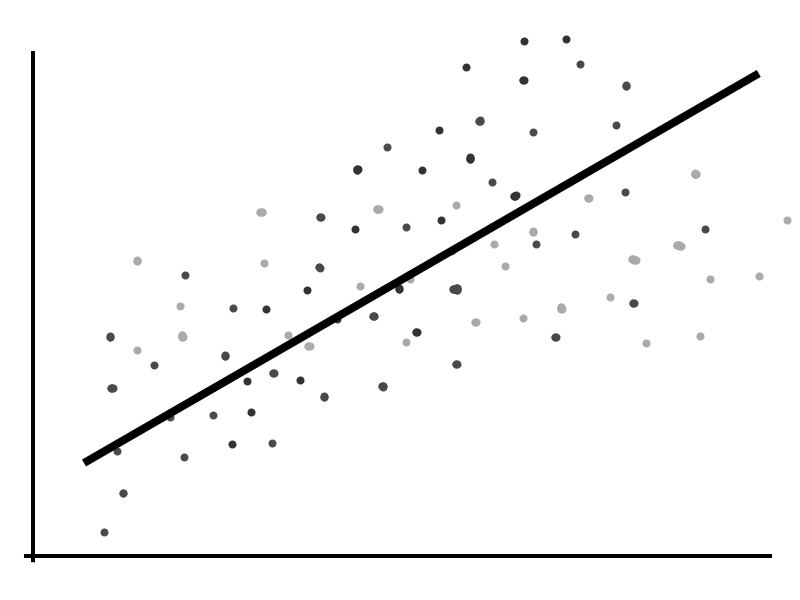
\includegraphics[width=3.125in,height=\textheight]{img/rcmodel001.png}
\caption{Simple OLS}
\end{figure}

\end{frame}

\begin{frame}{M: Empirical Framework (Intuition) II\}}
\protect\hypertarget{m-empirical-framework-intuition-ii}{}

\begin{figure}
\centering
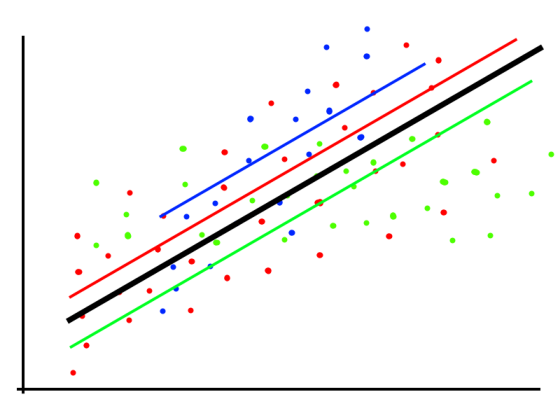
\includegraphics[width=3.125in,height=\textheight]{img/rcmodel002.png}
\caption{Multiple OLS with homogeneous return to Educ}
\end{figure}

\end{frame}

\begin{frame}{M: Empirical Framework (Intuition) III\}}
\protect\hypertarget{m-empirical-framework-intuition-iii}{}

\begin{figure}
\centering
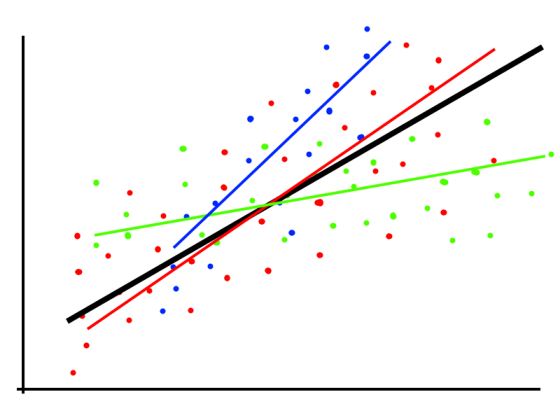
\includegraphics[width=3.125in,height=\textheight]{img/rcmodel003.png}
\caption{Correlated Random Coefficient Model}
\end{figure}

\end{frame}

\begin{frame}{M: Distinction to conventional methods\}}
\protect\hypertarget{m-distinction-to-conventional-methods}{}

\begin{itemize}
\item
  OLS

  \begin{itemize}
  \tightlist
  \item
    ability and ``background'' bias
  \end{itemize}
\item
  IV Methods:

  \begin{itemize}
  \tightlist
  \item
    suitable if assume homogeneous returns to education.
  \item
    if education is correlated with \textbf{unobserved individual
    heterogeneity}, IV methods may fail to identity APE.
  \item
    alternative: \textbf{L}ocal \textbf{A}verage \textbf{T}reatment
    \textbf{E}ffect if interested in effect of educational policy
    reforms.
  \end{itemize}
\end{itemize}

\end{frame}

\begin{frame}{M: Conditional Mean Independence\}}
\protect\hypertarget{m-conditional-mean-independence}{}

According to Wooldridge (2004, pg.7), \textbf{APE} is identified if:
\[E (\ln Y_i \mid a_i, b_i, S_i, X_i,) = E (\ln Y_i \mid a_i, b_i, S_i) = a_i+b_i S_i \qquad (A.1)\]
\[E(S_i \mid a_i, b_i, X_i) = E(S_i \mid X_i) ~~\text{and}~~ \mathrm{Var}(S_i \mid 
a_i, b_i, X_i) = \mathrm{Var} (S_i \mid X_i) \qquad (A.2)\]

\begin{itemize}
\tightlist
\item
  (A.1): Redundancy of \(X_i\) given \(a_i\) and \(b_i\) and \(S_i\).
\item
  (A.2): In the first two conditional moments of \(S_i\), \(a_i\) and
  \(b_i\) are redundant --\textgreater{} ``Staying longer in Education
  is determined by \(X\) covariates''.
\item
  Basically: \(X_i\) should be ``good predictors'' of treatment \(S_i\)
  (Wooldridge 2004, pg.7).
\end{itemize}

\end{frame}

\begin{frame}{M: Estimator for \(\beta\) and GLM\}}
\protect\hypertarget{m-estimator-for-beta-and-glm}{}

The \textbf{APE} can be estimated by:

\[\hat \beta = \frac{1}{N} \sum_{i=1}^N \left( \left( S_i - \hat E (S_i \mid X_i) \ln Y_i \right) \middle/
\hat{Var}(S_i \mid X_i)\right)\]

\[E(S_i \mid X_i ) = e^{\gamma X_i}  ~~~\text{and}~~~ Var(S_i \mid X_i ) = \sigma^2e^{\gamma X_i}\]
Where \(\sigma^2\) can be consistently estimated by the mean of squared
Pearson residuals and standard errors are bootstrapped.

\end{frame}

\begin{frame}[allowframebreaks]{L: Control Function Approach}
\protect\hypertarget{l-control-function-approach}{}

\begin{itemize}
\tightlist
\item
  Based on proposition by Garen (1984).
\item
  CF approach can identify APE in heterogeneous returns while standard
  IV approach may not.
\item
  Similar to Heckman two-step estimator.
\item
  Models schooling choice explicitly in first step
\end{itemize}

\textbf{First step}: modelling schooling choice

\[S_i = c'X_i + dZ_i + v_i ~~\text{with}~~ E(v_i \mid Z_i, X_i) = 0\]
where:

\begin{itemize}
\item
  \(X_i\) and \(Z_i\) influence the educational decision.
\item
  \(v_i\): Error term incorporating unobserved determinants of education
  choice.
\item
  \(Z_i\): Exclusion restriction (instrument).
\item
  \(v_i\), \(\varepsilon_{ai}\) and \(\varepsilon_{bi}\) are normally
  distributed with zero means and positive variances, that are possibly
  correlated
\item
  \(v_i\) is positive if an individual acquires higher education than
  expected conditional on observed characteristics
\end{itemize}

\textbf{Second step}: augmented wage equation
\[\ln Y_i = a_i + \beta S_i + \gamma_1 v_i + \gamma_2 V_iS_i + w_i\]
where:

\begin{itemize}
\item
  \(\gamma_1\) and \(\gamma_2\) are the \textbf{control functions}

  \begin{itemize}
  \item
    \(\gamma_1 = cov(\varepsilon_{ai}, v_i) /var(v_i)\)
  \item
    \(\gamma_2 = cov(\varepsilon_{bi}, v_i) /var(v_i)\)
  \end{itemize}
\item
  \(E(w_i \mid X_i, S_i, v_i) = 0\) (as shown in Heckman / Robb, 1985)
\end{itemize}

\end{frame}

\begin{frame}{L: Control Function Approach III}
\protect\hypertarget{l-control-function-approach-iii}{}

Interpretation of the coefficients of the control functions

\begin{itemize}
\tightlist
\item
  \(\gamma_1\) measures the effect of those unobserved factors that led
  to over- or under-achievement in education on the wage

  \begin{itemize}
  \tightlist
  \item
    Thus, if \(\gamma_1\) is positive, the unobserved factors affect
    schooling \emph{and} wages positively
  \end{itemize}
\item
  \(\gamma_2\) describes how this effect changes with increasing levels
  of education

  \begin{itemize}
  \tightlist
  \item
    Positive coefficient would indicate that those with unexpected
    educational ``over-achievement'' tend to earn higher wages
  \end{itemize}
\end{itemize}

\end{frame}

\hypertarget{replication-and-comparison}{%
\section{Replication and Comparison}\label{replication-and-comparison}}

\hypertarget{replication-and-comparison-1}{%
\subsection{Replication and
Comparison}\label{replication-and-comparison-1}}

\begin{frame}{L: Set-up}
\protect\hypertarget{l-set-up}{}

\begin{itemize}
\tightlist
\item
  We use the same sample: West Germans (not foreign-born or
  self-employed) between 25 and 60 years who work full-time
\item
  We have less observations than Gebel and Pfeiffer (2010) per survey
  year after we delete all observations with missing values
\item
  Yet, we extend the observation period until 2016
\item
  Three estimation methods: OLS, CMI CF
\item
  control variables: age and age squared, gender, father's education,
  mother's education, father's occupation, rural or urban household,
  number of siblings (as instrument)
\end{itemize}

\end{frame}

\begin{frame}{M: Stata Implementation (CMI)}
\protect\hypertarget{m-stata-implementation-cmi}{}

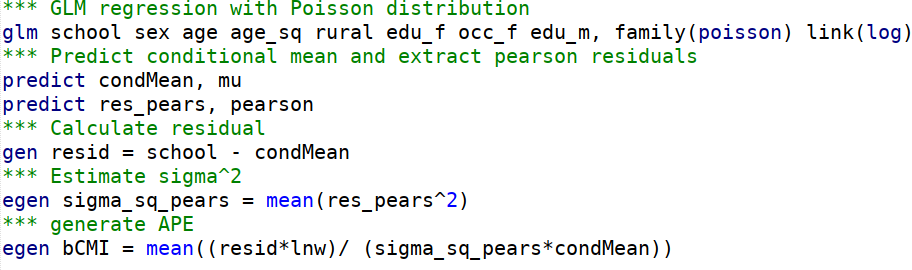
\includegraphics{./img/code_CMI.png}

\end{frame}

\begin{frame}{M: Stata Implementation (Bootstrapping)}
\protect\hypertarget{m-stata-implementation-bootstrapping}{}

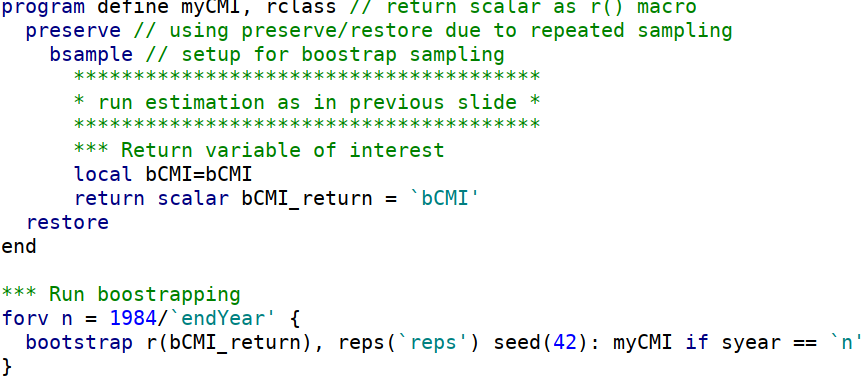
\includegraphics{./img/code_bootstrapping.png}

\end{frame}

\begin{frame}{L: Stata Implementation (CF)}
\protect\hypertarget{l-stata-implementation-cf}{}

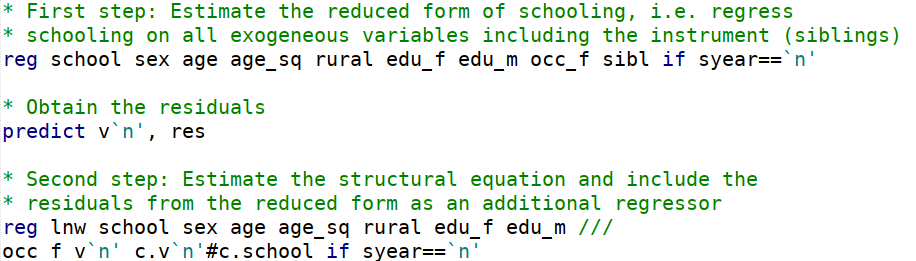
\includegraphics{./img/code_CF.png}

\end{frame}

\hypertarget{results}{%
\subsection{Results}\label{results}}

\begin{frame}{M: Results Comparison I\}}
\protect\hypertarget{m-results-comparison-i}{}

\begin{figure}
\centering
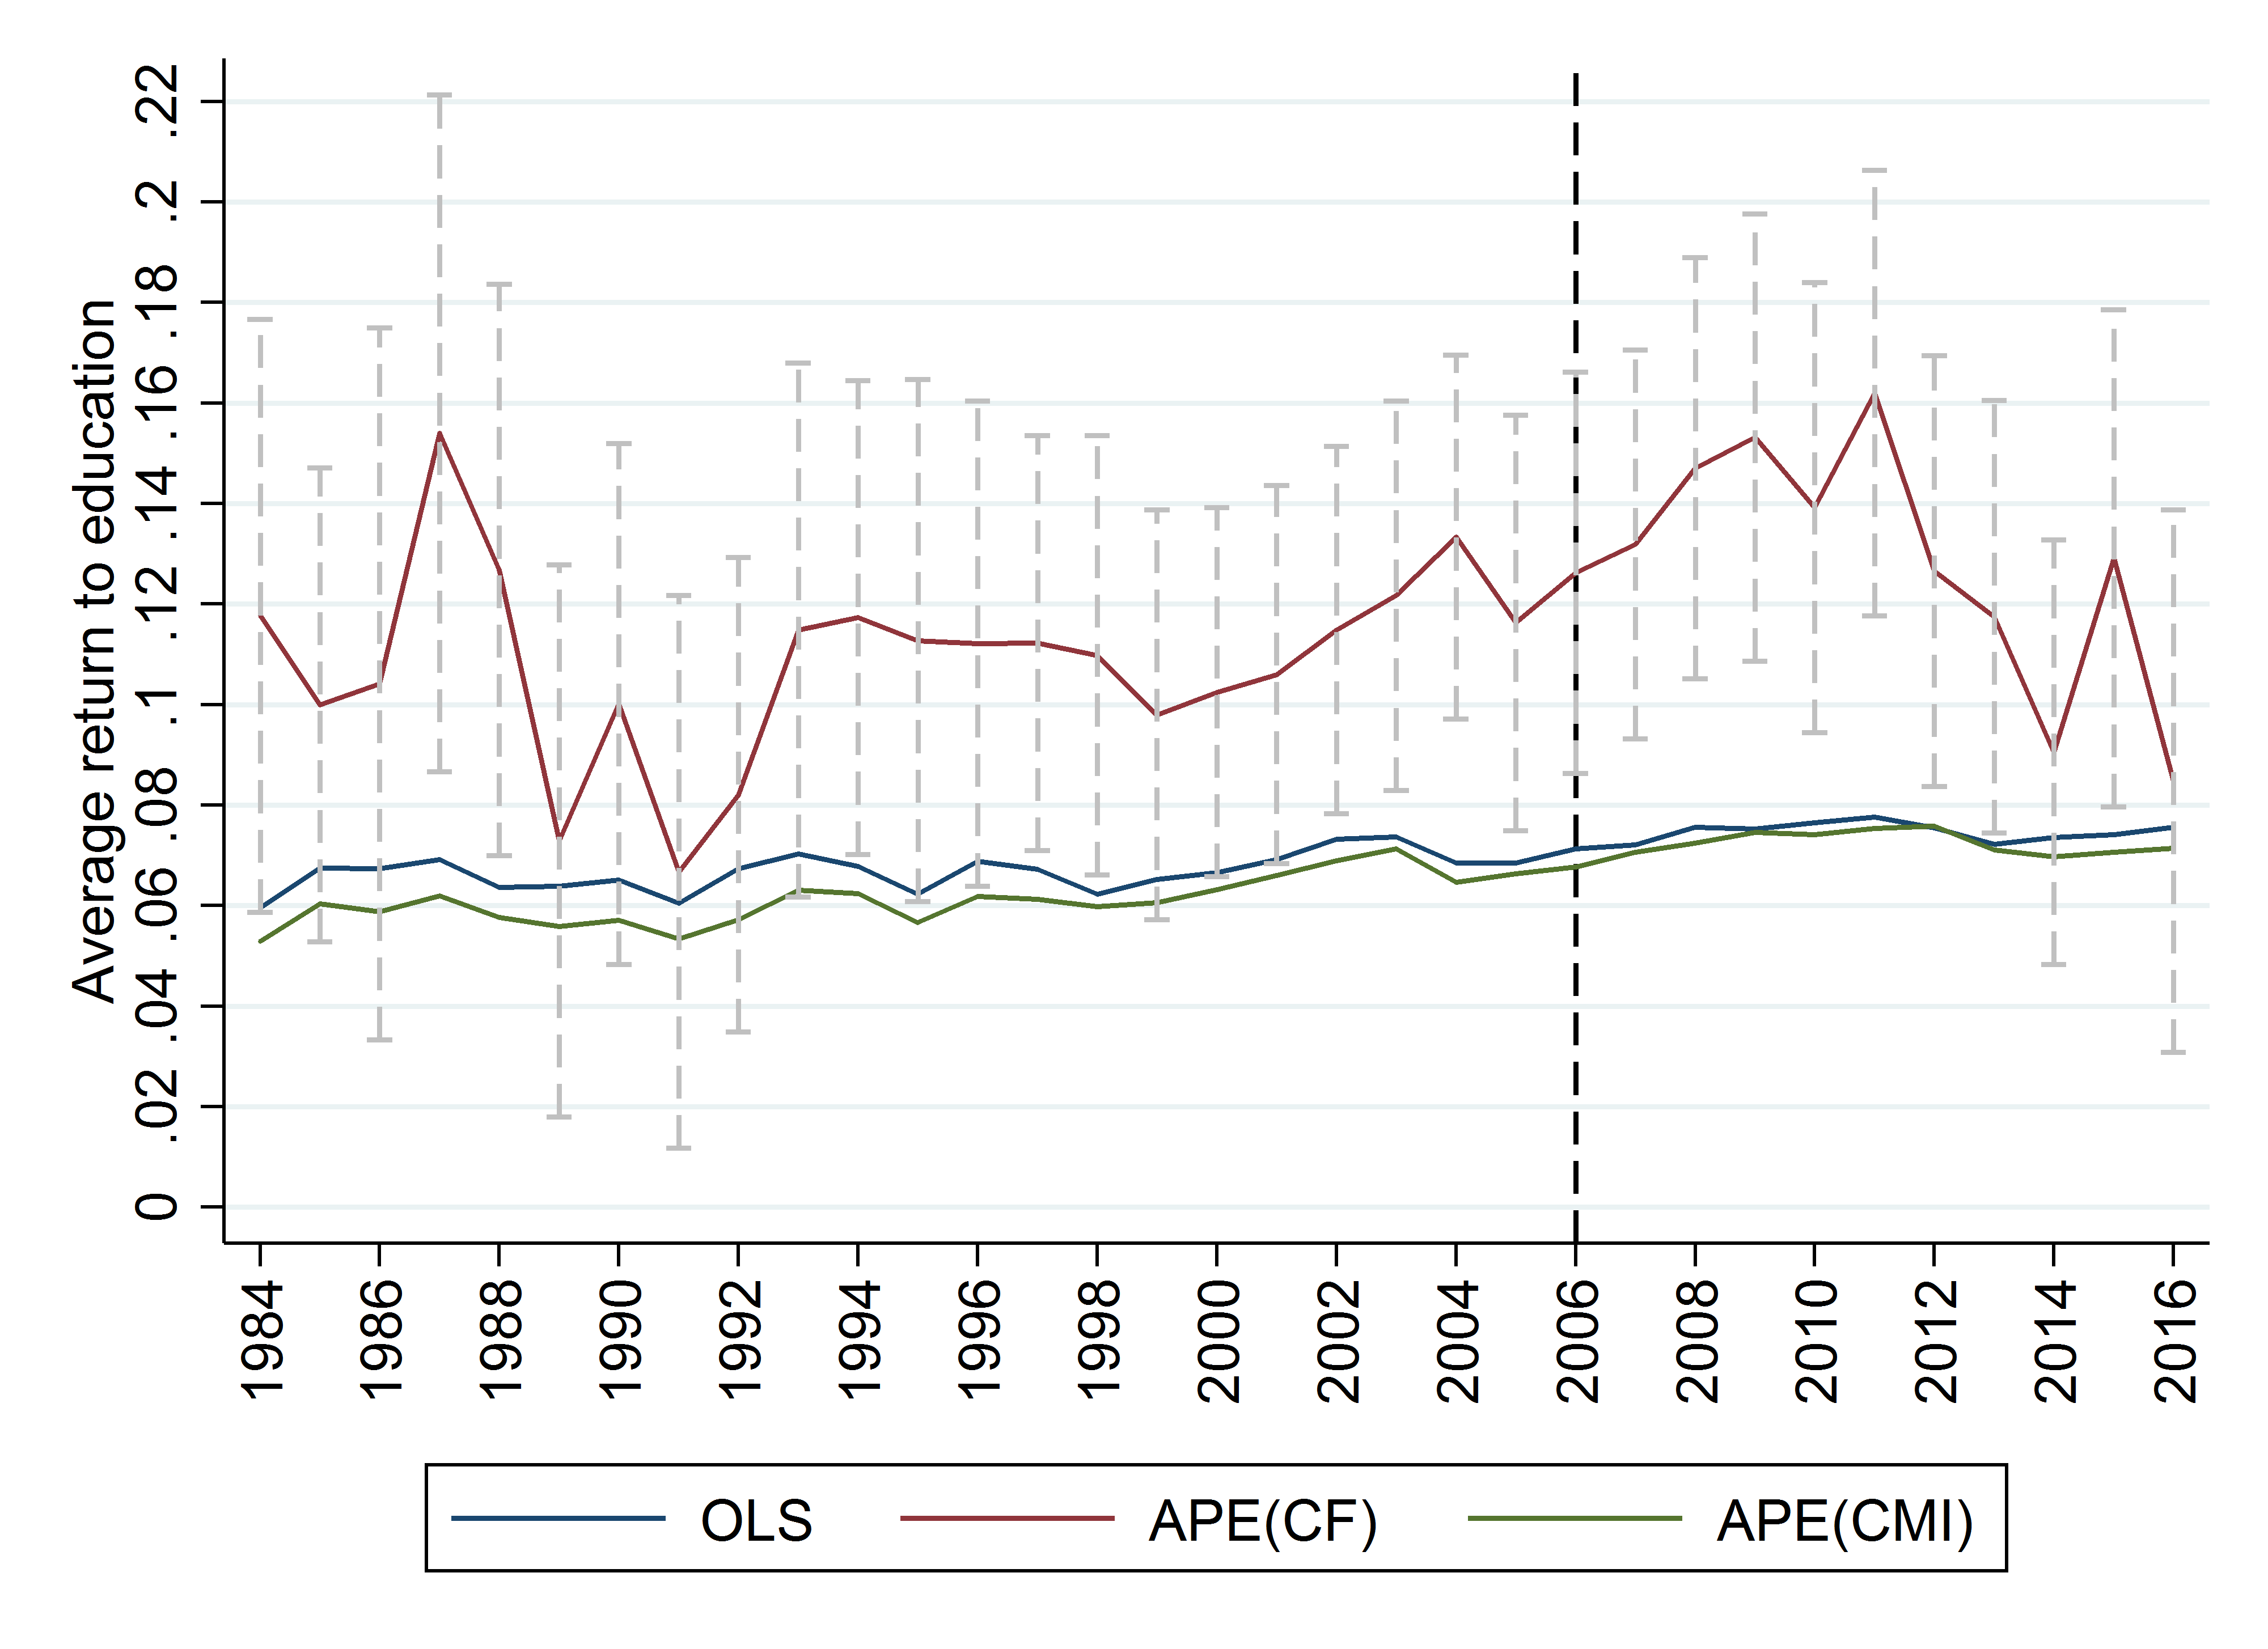
\includegraphics[width=\textwidth,height=2.60417in]{img/results.png}
\caption{Replication results: Comparison between OLS, CMI and CF
approaches}
\end{figure}

\end{frame}

\begin{frame}{M: Results Comparison II\}}
\protect\hypertarget{m-results-comparison-ii}{}

\begin{figure}
\centering
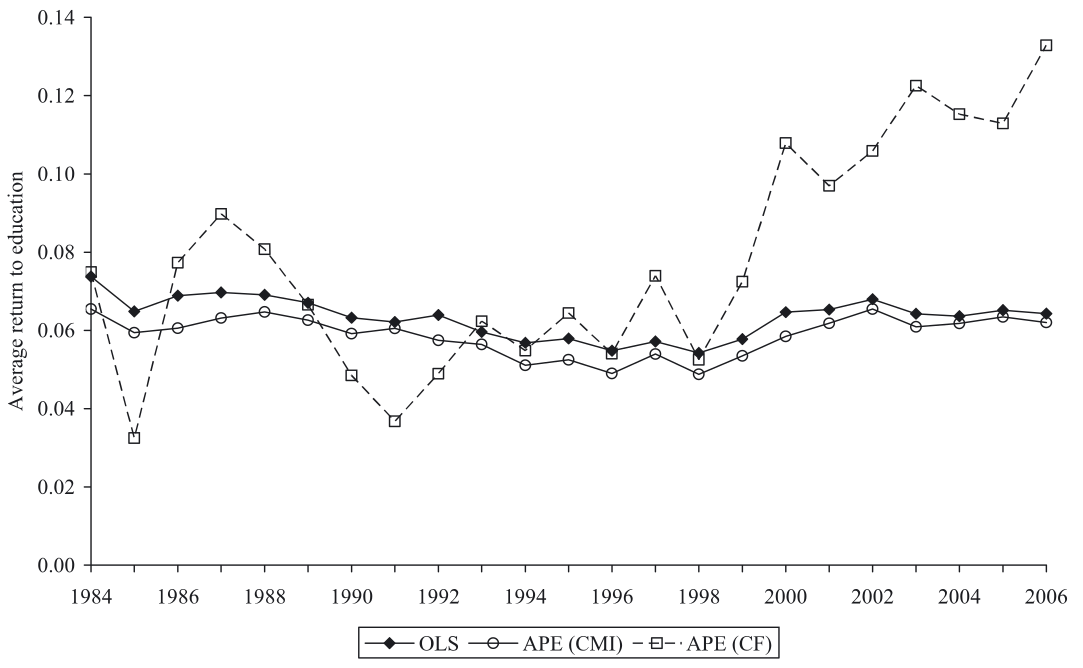
\includegraphics[width=\textwidth,height=2.60417in]{img/OLS_CMI_CF_GB2010.png}
\caption{Original Results (GP 2010, pg.30)}
\end{figure}

\end{frame}

\begin{frame}{M: Estimated returns on education}
\protect\hypertarget{m-estimated-returns-on-education}{}

\begin{itemize}
\tightlist
\item
  Estimates from OLS and CMI are similar, yet, CMI produces lower
  estimates which points to a positive self-selection bias
\item
  Generally, CF estimates are much more volatile and less precise
\end{itemize}

Differences between replicated and original estimations

\begin{itemize}
\tightlist
\item
  Our OLS estimates are on average larger than those of Gebel and
  Pfeiffer (2010) by 0.004 percentage points
\item
  Our CMI estimates are on average larger than those of Gebel and
  Pfeiffer (2010) by 0.002 percentage points (first years lower, than
  larger)
\item
  Our CF estimates are on average significantly larger by 0.032
  percentage points, though the divergence gets smaller from 2000
  onwards
\end{itemize}

\end{frame}

\begin{frame}[allowframebreaks]{L: Control function estimates}
\protect\hypertarget{l-control-function-estimates}{}

Instrumental variable in first step

\begin{itemize}
\tightlist
\item
  \emph{Number of siblings} is significant at the 0.1\% level for all
  years
\item
  As expected, the number of siblings has a negative impact on the years
  of schooling (the estimates range between -0.13 and -0.23)
\item
  We would assume that the instrument does not directly affect the error
  term in the wage equation
\end{itemize}

Coefficients of the control functions

\begin{itemize}
\tightlist
\item
  \(\gamma_1\) is negative for majority of years, yet very small and
  insignificant in all years

  \begin{itemize}
  \tightlist
  \item
    Gebel and Pfeiffer (2010) estimate a positive coefficient in the
    1980s and 1990s - but also insignificant
  \end{itemize}
\item
  \(\gamma_2\) is negative and close to zero for most years

  \begin{itemize}
  \tightlist
  \item
    Indicates that those with unexpectedly high education have lower
    returns to education
  \item
    Similarly, they are only slightly significant in the 1980s, and
    stronger significant in the early 2000s
  \item
    The estimates are very similar to those of Gebel and Pfeiffer (2010)
  \end{itemize}
\item
  that both coefficients are (mostly) negative hints that educational
  expansion caused more ``less abled'' to achieve higher education
\end{itemize}

\end{frame}

\begin{frame}{L: Results: Control Function (replication)}
\protect\hypertarget{l-results-control-function-replication}{}

\begingroup\fontsize{7}{9}\selectfont

\begin{longtable}[t]{rrrrrrrrr}
\caption{\label{tab:unnamed-chunk-2}Summary of Control Function estimates (replication)}\\
\toprule
\multicolumn{1}{c}{ } & \multicolumn{2}{c}{First Stage} & \multicolumn{6}{c}{Second Stage} \\
\cmidrule(l{2pt}r{2pt}){2-3} \cmidrule(l{2pt}r{2pt}){4-9}
\multicolumn{1}{c}{ } & \multicolumn{2}{c}{IV: Nr. of Siblings} & \multicolumn{3}{c}{$v_i$} & \multicolumn{3}{c}{$v_i S_i$} \\
\cmidrule(l{2pt}r{2pt}){2-3} \cmidrule(l{2pt}r{2pt}){4-6} \cmidrule(l{2pt}r{2pt}){7-9}
year & coef. & s.e. & coef. & s.e. & p & coef. & s.e. & p\\
\midrule
\endfirsthead
\caption[]{Summary of Control Function estimates (replication) \textit{(continued)}}\\
\toprule
\multicolumn{1}{c}{ } & \multicolumn{2}{c}{First Stage} & \multicolumn{6}{c}{Second Stage} \\
\cmidrule(l{2pt}r{2pt}){2-3} \cmidrule(l{2pt}r{2pt}){4-9}
\multicolumn{1}{c}{ } & \multicolumn{2}{c}{IV: Nr. of Siblings} & \multicolumn{3}{c}{$v_i$} & \multicolumn{3}{c}{$v_i S_i$} \\
\cmidrule(l{2pt}r{2pt}){2-3} \cmidrule(l{2pt}r{2pt}){4-6} \cmidrule(l{2pt}r{2pt}){7-9}
year & coef. & s.e. & coef. & s.e. & p & coef. & s.e. & p\\
\midrule
\endhead
\
\endfoot
\bottomrule
\endlastfoot
1984 & -0.163 & 0.035 & -0.019 & 0.036 & 0.601 & -0.003 & 0.001 & 0.027\\
1985 & -0.191 & 0.036 & 0.005 & 0.030 & 0.864 & -0.003 & 0.001 & 0.024\\
1986 & -0.129 & 0.034 & -0.039 & 0.041 & 0.344 & -0.001 & 0.001 & 0.681\\
1987 & -0.133 & 0.033 & -0.064 & 0.039 & 0.105 & -0.002 & 0.001 & 0.141\\
1988 & -0.150 & 0.034 & -0.031 & 0.034 & 0.365 & -0.003 & 0.001 & 0.038\\
\addlinespace
1989 & -0.153 & 0.033 & 0.018 & 0.033 & 0.590 & -0.002 & 0.001 & 0.056\\
1990 & -0.164 & 0.032 & -0.027 & 0.032 & 0.404 & -0.001 & 0.001 & 0.341\\
1991 & -0.167 & 0.033 & 0.014 & 0.034 & 0.685 & -0.002 & 0.001 & 0.152\\
1992 & -0.178 & 0.032 & -0.007 & 0.030 & 0.808 & -0.001 & 0.001 & 0.298\\
1993 & -0.162 & 0.033 & -0.033 & 0.033 & 0.311 & -0.001 & 0.001 & 0.264\\
\addlinespace
1994 & -0.176 & 0.034 & -0.035 & 0.029 & 0.233 & -0.001 & 0.001 & 0.225\\
1995 & -0.172 & 0.036 & -0.026 & 0.032 & 0.422 & -0.002 & 0.001 & 0.077\\
1996 & -0.195 & 0.037 & -0.015 & 0.031 & 0.624 & -0.003 & 0.001 & 0.058\\
1997 & -0.214 & 0.038 & -0.030 & 0.027 & 0.268 & -0.002 & 0.001 & 0.225\\*
\end{longtable}\endgroup{}

\end{frame}

\begin{frame}{?: Heterogenous returns to education by gender I}
\protect\hypertarget{heterogenous-returns-to-education-by-gender-i}{}

\begin{figure}
\centering
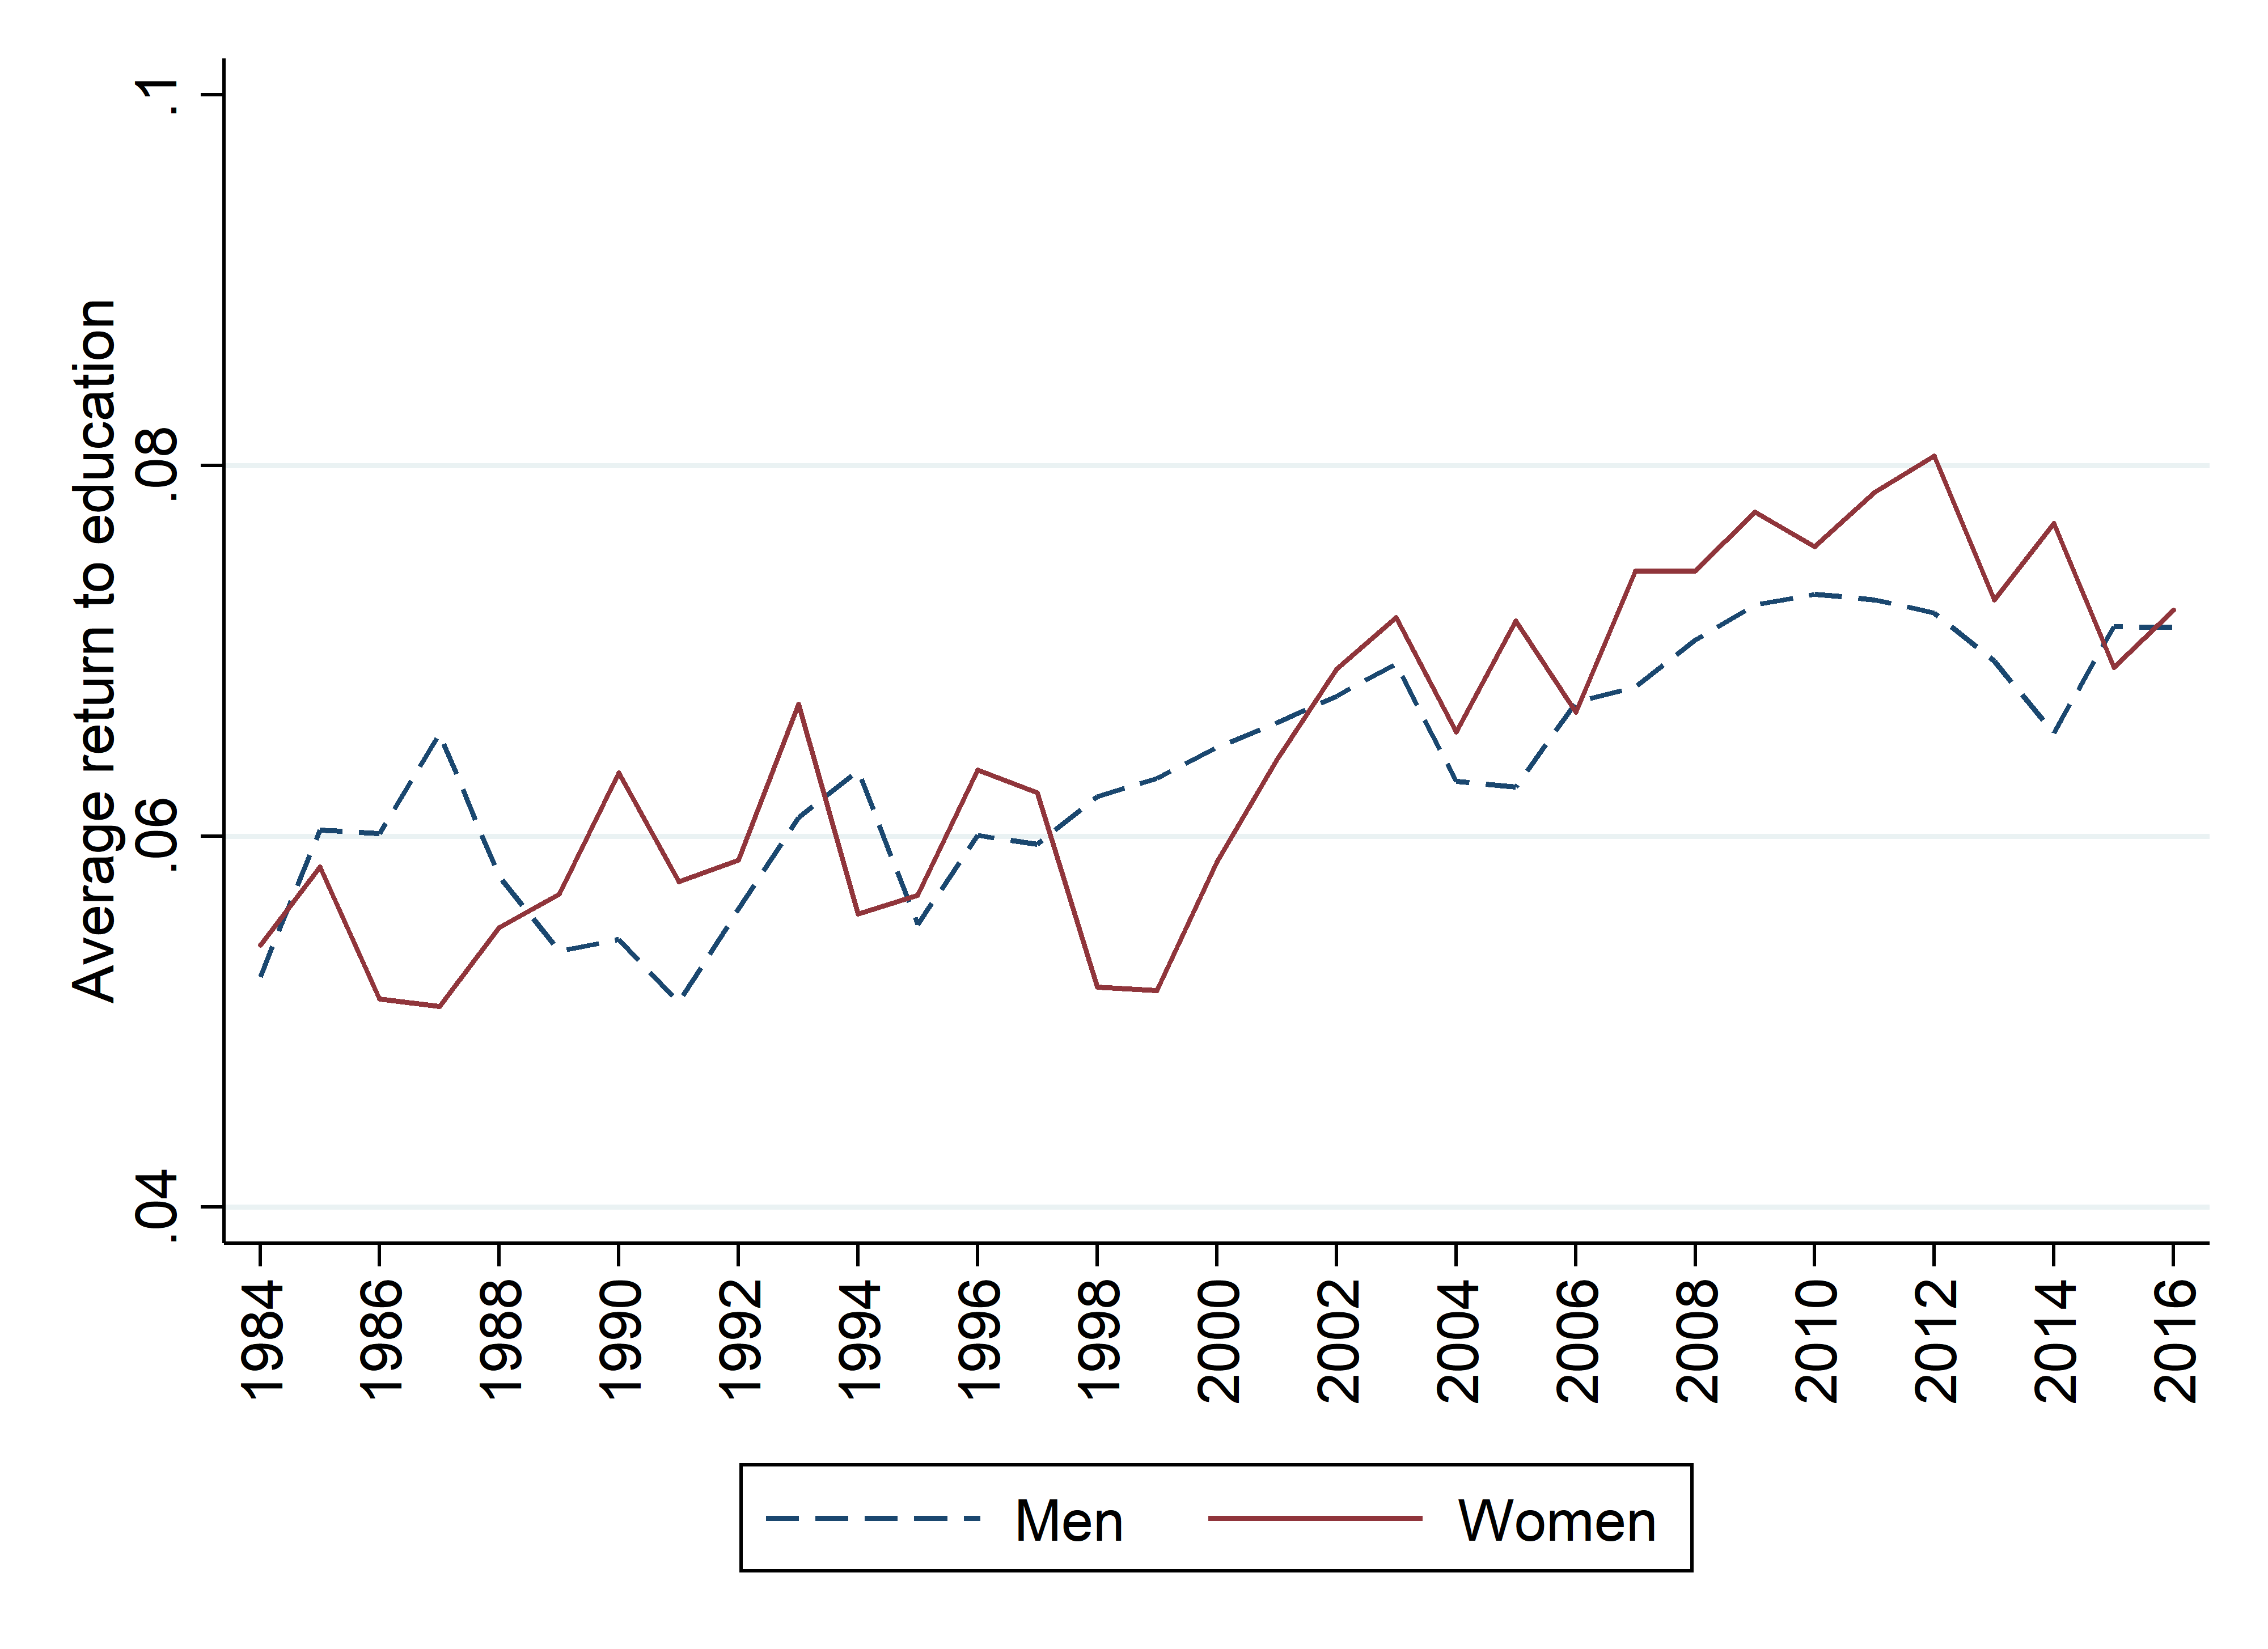
\includegraphics[width=\textwidth,height=2.60417in]{img/results_sex.png}
\caption{Replication results: \textbf{APE} by gender (CMI)}
\end{figure}

\end{frame}

\begin{frame}{?: Heterogenous returns to education by gender II}
\protect\hypertarget{heterogenous-returns-to-education-by-gender-ii}{}

\begin{figure}
\centering
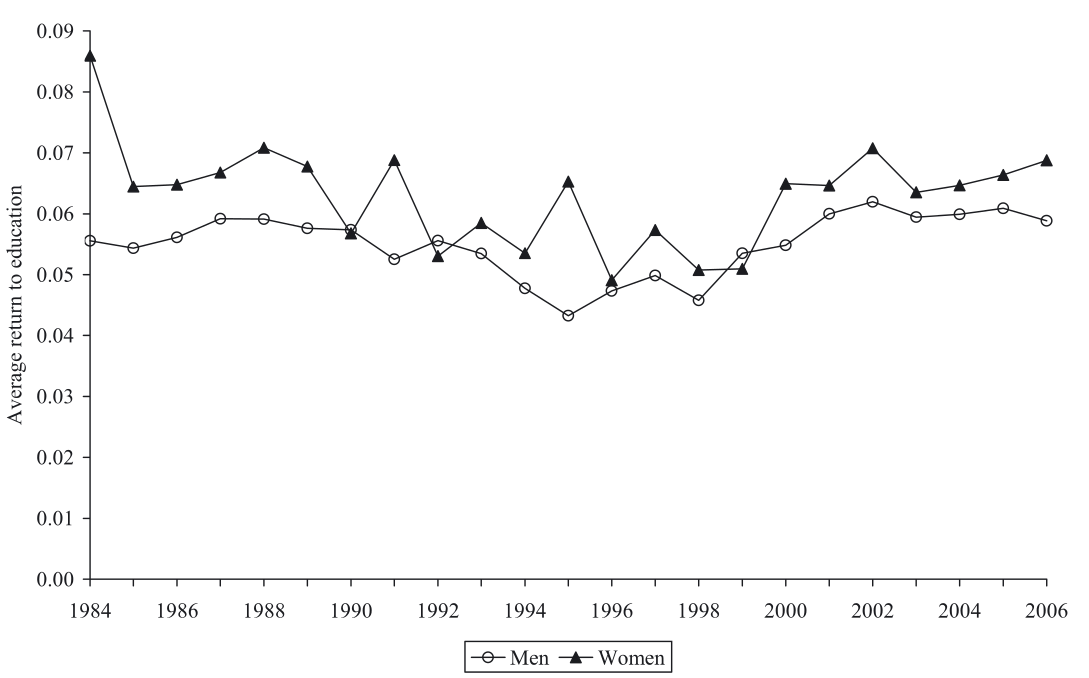
\includegraphics[width=\textwidth,height=2.60417in]{img/GP2010_CMI_gender.png}
\caption{Original Results \textbf{APE} by gender (CMI) (GP 2010, pg.34}
\end{figure}

\end{frame}

\hypertarget{conclusion}{%
\subsection{Conclusion}\label{conclusion}}

\begin{frame}{L: Conclusion}
\protect\hypertarget{l-conclusion}{}

\begin{itemize}
\item
  CMI - no analytical standard errors - only identifies APE.
\item
  CF - requires further distributional assumptions on error terms -
  requires valid and relevant ``instrument'' - estimates are very
  imprecise
\end{itemize}

\end{frame}

\hypertarget{the-end}{%
\subsection{The end}\label{the-end}}

\begin{frame}[allowframebreaks]{Appendix}
\protect\hypertarget{appendix}{}

\begingroup\fontsize{7}{9}\selectfont

\begin{longtable}[t]{rrrrrrrl}
\caption{\label{tab:unnamed-chunk-3}Summary original results GB(2010).}\\
\toprule
year & OLS & s.e. (OLS) & CMI & s.e. (CMI) & CF & s.e. (CF) & obs\\
\midrule
\endfirsthead
\caption[]{Summary original results GB(2010). \textit{(continued)}}\\
\toprule
year & OLS & s.e. (OLS) & CMI & s.e. (CMI) & CF & s.e. (CF) & obs\\
\midrule
\endhead
\
\endfoot
\bottomrule
\endlastfoot
1984 & 0.074 & 0.004 & 0.066 & 0.004 & 0.075 & 0.079 & 1.545\\
1985 & 0.065 & 0.004 & 0.059 & 0.004 & 0.032 & 0.131 & 1.600\\
1986 & 0.069 & 0.004 & 0.061 & 0.004 & 0.077 & 0.091 & 1.682\\
1987 & 0.070 & 0.004 & 0.063 & 0.004 & 0.090 & 0.048 & 1.775\\
1988 & 0.069 & 0.004 & 0.065 & 0.004 & 0.081 & 0.041 & 1.798\\
\addlinespace
1989 & 0.067 & 0.003 & 0.063 & 0.004 & 0.067 & 0.038 & 1.922\\
1990 & 0.063 & 0.003 & 0.059 & 0.004 & 0.048 & 0.031 & 2.007\\
1991 & 0.062 & 0.003 & 0.060 & 0.004 & 0.037 & 0.030 & 2.122\\
1992 & 0.064 & 0.003 & 0.057 & 0.004 & 0.049 & 0.027 & 2.107\\
1993 & 0.060 & 0.003 & 0.057 & 0.004 & 0.062 & 0.026 & 2.124\\
\addlinespace
1994 & 0.057 & 0.003 & 0.051 & 0.004 & 0.055 & 0.022 & 2.082\\
1995 & 0.058 & 0.003 & 0.053 & 0.004 & 0.064 & 0.024 & 2.075\\
1996 & 0.055 & 0.003 & 0.049 & 0.004 & 0.054 & 0.025 & 2.057\\
1997 & 0.057 & 0.003 & 0.054 & 0.003 & 0.074 & 0.025 & 2.011\\
1998 & 0.054 & 0.003 & 0.049 & 0.003 & 0.053 & 0.021 & 2.145\\
\addlinespace
1999 & 0.058 & 0.003 & 0.054 & 0.003 & 0.072 & 0.023 & 2.163\\
2000 & 0.065 & 0.002 & 0.059 & 0.003 & 0.108 & 0.024 & 3.965\\
2001 & 0.065 & 0.002 & 0.062 & 0.003 & 0.097 & 0.022 & 3.961\\
2002 & 0.068 & 0.003 & 0.066 & 0.003 & 0.106 & 0.030 & 3.668\\
2003 & 0.064 & 0.003 & 0.062 & 0.003 & 0.123 & 0.028 & 3.476\\
\addlinespace
2004 & 0.064 & 0.003 & 0.062 & 0.003 & 0.115 & 0.030 & 3.366\\
2005 & 0.065 & 0.003 & 0.064 & 0.003 & 0.113 & 0.032 & 3.220\\
2006 & 0.064 & 0.003 & 0.063 & 0.003 & 0.133 & 0.033 & 3.477\\*
\end{longtable}\endgroup{}

\begingroup\fontsize{7}{9}\selectfont

\begin{longtable}[t]{rrrrrrrl}
\caption{\label{tab:unnamed-chunk-4}Summary replication results.}\\
\toprule
year & OLS & s.e. (OLS) & CMI & s.e. (CMI) & CF & s.e. (CF) & obs\\
\midrule
\endfirsthead
\caption[]{Summary replication results. \textit{(continued)}}\\
\toprule
year & OLS & s.e. (OLS) & CMI & s.e. (CMI) & CF & s.e. (CF) & obs\\
\midrule
\endhead
\
\endfoot
\bottomrule
\endlastfoot
1984 & 0.060 & 0.004 & 0.030 & 0.118 & 0.053 & 0.006 & 1.448\\
1985 & 0.067 & 0.003 & 0.024 & 0.100 & 0.060 & 0.005 & 1.412\\
1986 & 0.067 & 0.004 & 0.036 & 0.104 & 0.059 & 0.006 & 1.463\\
1987 & 0.069 & 0.004 & 0.034 & 0.154 & 0.062 & 0.005 & 1.489\\
1988 & 0.064 & 0.003 & 0.029 & 0.127 & 0.058 & 0.005 & 1.476\\
\addlinespace
1989 & 0.064 & 0.003 & 0.028 & 0.073 & 0.056 & 0.005 & 1.553\\
1990 & 0.065 & 0.003 & 0.026 & 0.100 & 0.057 & 0.005 & 1.571\\
1991 & 0.060 & 0.004 & 0.028 & 0.067 & 0.053 & 0.005 & 1.602\\
1992 & 0.067 & 0.003 & 0.024 & 0.082 & 0.057 & 0.005 & 1.555\\
1993 & 0.070 & 0.004 & 0.027 & 0.115 & 0.063 & 0.005 & 1.527\\
\addlinespace
1994 & 0.068 & 0.003 & 0.024 & 0.117 & 0.062 & 0.005 & 1.491\\
1995 & 0.062 & 0.003 & 0.026 & 0.113 & 0.057 & 0.005 & 1.444\\
1996 & 0.069 & 0.003 & 0.025 & 0.112 & 0.062 & 0.005 & 1.383\\
1997 & 0.067 & 0.003 & 0.021 & 0.112 & 0.061 & 0.005 & 1.285\\
1998 & 0.062 & 0.003 & 0.022 & 0.110 & 0.060 & 0.005 & 1.452\\
\addlinespace
1999 & 0.065 & 0.003 & 0.021 & 0.098 & 0.061 & 0.005 & 1.452\\
2000 & 0.067 & 0.003 & 0.019 & 0.102 & 0.063 & 0.004 & 2.701\\
2001 & 0.069 & 0.003 & 0.019 & 0.106 & 0.066 & 0.004 & 2.659\\
2002 & 0.073 & 0.003 & 0.019 & 0.115 & 0.069 & 0.004 & 2.818\\
2003 & 0.074 & 0.003 & 0.020 & 0.122 & 0.071 & 0.004 & 2.741\\
\addlinespace
2004 & 0.069 & 0.003 & 0.018 & 0.133 & 0.065 & 0.004 & 2.558\\
2005 & 0.069 & 0.003 & 0.021 & 0.116 & 0.066 & 0.004 & 2.457\\
2006 & 0.071 & 0.003 & 0.020 & 0.126 & 0.068 & 0.004 & 2.525\\
2007 & 0.072 & 0.003 & 0.020 & 0.132 & 0.071 & 0.004 & 2.462\\
2008 & 0.076 & 0.003 & 0.021 & 0.147 & 0.072 & 0.005 & 2.316\\
\addlinespace
2009 & 0.075 & 0.003 & 0.023 & 0.153 & 0.075 & 0.004 & 2.367\\
2010 & 0.077 & 0.003 & 0.023 & 0.139 & 0.074 & 0.005 & 2.183\\
2011 & 0.078 & 0.003 & 0.023 & 0.162 & 0.075 & 0.004 & 2.523\\
2012 & 0.076 & 0.003 & 0.022 & 0.127 & 0.076 & 0.004 & 2.493\\
2013 & 0.072 & 0.003 & 0.022 & 0.117 & 0.071 & 0.004 & 2.477\\
\addlinespace
2014 & 0.074 & 0.003 & 0.022 & 0.091 & 0.070 & 0.004 & 2.353\\
2015 & 0.074 & 0.003 & 0.025 & 0.129 & 0.071 & 0.005 & 2.147\\
2016 & 0.076 & 0.003 & 0.028 & 0.085 & 0.071 & 0.005 & 1.971\\*
\end{longtable}\endgroup{}

\end{frame}

\end{document}
